\documentclass[a4paper,twocolumn,11pt,unpublished]{quantumarticle}
\pdfoutput=1
\usepackage[utf8]{inputenc}
\usepackage[english]{babel}
\usepackage[T1]{fontenc}
\usepackage{amsmath,amssymb,amsthm,mathtools}
\usepackage{booktabs}
\usepackage{supertabular}
\usepackage{graphicx}
\usepackage{microtype}
\usepackage{hyperref}
\usepackage[numbers,sort&compress]{natbib}
\usepackage{xcolor}
\usepackage{quantikz}

\newtheorem{proposition}{Proposition}
\newcommand{\bits}{\{0,1\}}
\newcommand{\E}{\mathbb{E}}
\newcommand{\mmd}{\operatorname{MMD}}
\newcommand{\TVD}{\operatorname{TVD}}
\newcommand{\supp}{\operatorname{supp}}
\makeatletter
\newcommand{\tableinput}[1]{\@@input #1 }
\makeatother
\definecolor{paperblue}{HTML}{0072B2}
\definecolor{paperorange}{HTML}{D55E00}
\definecolor{papergreen}{HTML}{009E73}
\definecolor{paperpurple}{HTML}{CC79A7}

\newif\ifgaussianresults
\IfFileExists{generated/gaussian_claims.tex}{
  \gaussianresultstrue
  \input{generated/gaussian_claims}
}{
  \gaussianresultsfalse
  \newcommand{\GaussianAtomicModels}{0 of 1,020}
  \newcommand{\ProfileControlSupported}{pending}
  \newcommand{\ProfileControlMixed}{pending}
  \newcommand{\ProfileControlUnsupported}{pending}
  \newcommand{\ProfileLookupSupported}{pending}
  \newcommand{\ProfileLookupMixed}{pending}
  \newcommand{\ProfileLookupUnsupported}{pending}
  \newcommand{\ProfileMixtureSupported}{pending}
  \newcommand{\ProfileMixtureMixed}{pending}
  \newcommand{\ProfileMixtureUnsupported}{pending}
  \newcommand{\BitstringControlSupported}{pending}
  \newcommand{\BitstringControlMixed}{pending}
  \newcommand{\BitstringControlUnsupported}{pending}
  \newcommand{\BitstringLookupSupported}{pending}
  \newcommand{\BitstringLookupMixed}{pending}
  \newcommand{\BitstringLookupUnsupported}{pending}
  \newcommand{\HeadlineProfileControl}{pending}
  \newcommand{\HeadlineProfileBankGap}{pending}
  \newcommand{\HeadlineProfileLookup}{pending}
  \newcommand{\HeadlineProfileMixture}{pending}
  \newcommand{\HeadlineBitstringLookup}{pending}
}
\newif\ifcurieweissresults
\IfFileExists{generated/curie_weiss_claims.tex}{
  \curieweissresultstrue
}{
  \curieweissresultsfalse
}
\IfFileExists{generated/curie_weiss_effects.tex}{
  \newcommand{\curieweisseffectstablebody}{
    \tableinput{generated/curie_weiss_effects.tex}}
}{\newcommand{\curieweisseffectstablebody}{
  \multicolumn{6}{c}{Generated after campaign completion.}\\}}
\IfFileExists{generated/curie_weiss_response_table.tex}{
  \newcommand{\curieweissresponsetablebody}{
    \tableinput{generated/curie_weiss_response_table.tex}}
}{\newcommand{\curieweissresponsetablebody}{
  \multicolumn{10}{c}{Generated after campaign completion.}\\}}
\IfFileExists{generated/curie_weiss_mmd_bandwidths.tex}{
  \newcommand{\curieweissmmdtablebody}{
    \tableinput{generated/curie_weiss_mmd_bandwidths.tex}}
}{\newcommand{\curieweissmmdtablebody}{
  \multicolumn{5}{c}{Generated after campaign completion.}\\}}
\IfFileExists{generated/factorial_cells.tex}{
  \newcommand{\factorialtablebody}{\input{generated/factorial_cells}}
}{\newcommand{\factorialtablebody}{
  \multicolumn{6}{c}{Generated after campaign completion.}\\}}
\IfFileExists{generated/factorial_wins.tex}{
  \newcommand{\factorialwinstablebody}{\input{generated/factorial_wins}}
}{\newcommand{\factorialwinstablebody}{
  \multicolumn{5}{c}{Generated after campaign completion.}\\}}
\IfFileExists{generated/raw_bitstring_cells.tex}{
  \newcommand{\bitstringtablebody}{\input{generated/raw_bitstring_cells}}
}{\newcommand{\bitstringtablebody}{
  \multicolumn{6}{c}{Generated after campaign completion.}\\}}
\IfFileExists{generated/secondary_diagnostics.tex}{
  \newcommand{\secondarydiagnosticstablebody}{
    \input{generated/secondary_diagnostics}}
}{\newcommand{\secondarydiagnosticstablebody}{
  \multicolumn{8}{c}{Generated after campaign completion.}\\}}
\IfFileExists{generated/condition_count_cells.tex}{
  \newcommand{\conditioncounttablebody}{
    \input{generated/condition_count_cells}}
}{\newcommand{\conditioncounttablebody}{
  \multicolumn{9}{c}{Generated after campaign completion.}\\}}
\IfFileExists{generated/condition_count_per_condition.tex}{
  \newcommand{\conditioncountperconditiontablebody}{
    \input{generated/condition_count_per_condition}}
}{\newcommand{\conditioncountperconditiontablebody}{
  \multicolumn{7}{c}{Generated after campaign completion.}\\}}
\IfFileExists{generated/condition_count_intervals.tex}{
  \newcommand{\conditioncountintervalstablebody}{
    \input{generated/condition_count_intervals}}
}{\newcommand{\conditioncountintervalstablebody}{
  \multicolumn{6}{c}{Generated after campaign completion.}\\}}
\IfFileExists{generated/all_intervals.tex}{
  \newcommand{\allintervalstablebody}{\input{generated/all_intervals}}
}{\newcommand{\allintervalstablebody}{
  \multicolumn{4}{c}{Generated after campaign completion.}\\}}

\newcommand{\campaignfigure}[3]{%
  \begin{figure*}[t]
  \centering
  \IfFileExists{gaussian_figures/#1.pdf}{%
    \includegraphics[width=\textwidth]{gaussian_figures/#1.pdf}%
  }{\fbox{\parbox[c][40mm][c]{0.92\textwidth}{\centering
    Figure generated after complete immutable campaign finalization.}}}
  \caption{#2}
  \label{#3}
  \end{figure*}
}
\newcommand{\curieweissfigure}[3]{%
  \begin{figure*}[t]
  \centering
  \IfFileExists{curie_weiss_figures/#1.pdf}{%
    \includegraphics[width=\textwidth]{curie_weiss_figures/#1.pdf}%
  }{\fbox{\parbox[c][40mm][c]{0.92\textwidth}{\centering
    Generated only after all 270 immutable Curie--Weiss fits.}}}
  \caption{#2}
  \label{#3}
  \end{figure*}
}

\title{Conditional Generation with Classically Trainable IQP Circuits}
\author{Oriol Balló-Gimbernat}
\email{oriol.ballo@eurecat.org}
\affiliation{Eurecat, Centre Tecnològic de Catalunya, Barcelona, Spain}
\affiliation{Centre de Visió per Computador (CVC), Barcelona, Spain}
\affiliation{Universitat Autònoma de Barcelona (UAB), Barcelona, Spain}
\author{Emiliano Tolotti}
\email{emiliano.tolotti@unitn.it}
\affiliation{Department of Information Engineering and Computer Science,
University of Trento, Via Sommarive 9, 38123 Trento, Italy}

\begin{document}
\maketitle

\begin{abstract}
Quantum circuit Born machines offer expressive generative models, but it is
unclear how to make them conditional while preserving the structure that makes
some instantaneous quantum polynomial-time (IQP) circuits classically
trainable.  We preserve that structure with a simple idea: encode the condition in a product-state
input, while using the same compiled IQP circuit and the same learned phases
for every condition.  A single circuit then represents an entire conditional
distribution, and its kernel maximum mean discrepancy objective and gradients
remain expressible through classically estimable Pauli observables.  This
extends classically trainable IQP Born machines to conditional generation
without requiring classical simulation of the full output distribution during
optimization.  We study the model on a controlled generative task in which the
peak of a Gaussian distribution over Hamming weight moves continuously with
the condition.  A second benchmark asks whether the same mechanism follows
the temperature response of the Curie--Weiss model, whose magnetization law
changes from a central profile to an ordered bimodal profile.
\ifgaussianresults
Across 8--19 qubits and several target widths, the conditioned circuit moves
the generated Hamming-weight profile with the requested peak and consistently
outperforms an otherwise identical model that receives no condition.  This
behavior extends to peak locations not seen during training, demonstrating
within-range interpolation.  Separate circuits trained for individual peak
locations are usually more accurate, quantifying the fidelity cost of using
one shared circuit.  These results establish product-state conditioning as a
practical route from classically trainable IQP generation to conditional
generation on this benchmark.
\else
Numerical claims are intentionally absent until the immutable Gaussian
campaign is complete.
\fi
\ifcurieweissresults
On Curie--Weiss targets, conditioning improves over the no-condition control
at 12 and 16 spins but not at 8 spins.  Independently trained neighboring
models remain more accurate at every size, and an unrestricted phase model
outperforms the symmetry-tied model.  Thus the same mechanism produces a
temperature-dependent response, but does not by itself deliver high-fidelity
thermal generation near the unseen critical point or the cold endpoint.
\else
Curie--Weiss numerical claims remain disabled until all 270 declared fits and
exact evaluations are complete.
\fi
\end{abstract}

\section{Introduction}

Conditional generative models represent a family $q_\theta(x\mid c)$ rather
than a single probability law.  Quantum circuit Born machines (QCBMs) encode
discrete distributions directly in the measurement statistics of
parameterized quantum states and have been studied with likelihood-free,
kernel, and divergence-based objectives
\cite{liuDifferentiableLearning2018,benedettiGenerativeModeling2019,
gaoQuantumGenerativeModels2018,leadbeaterFDivergences2021}.  Conditional QCBMs have
also encoded external variables by data-reuploading rotations or additional
condition qubits
\cite{kissConditionalBornMachine2022,zengConditionalQCBM2023}.  Those works
establish that quantum generators can be conditioned; the unresolved question
here is whether conditioning can be added to the recently developed
\emph{classically trained} IQP Born machine without changing its compiled
sampling circuit or its trained phases from one condition to another.

The distinction between training and sampling is central to this question.
For commuting circuits, selected observables can be estimated classically
under structural assumptions even though approximate sampling from other IQP
families is linked to complexity-theoretic hardness
\cite{shepherdTemporallyUnstructured2009,nestSimulatingQuantumComputers2011,
niCommutingQuantumCircuits2012,
bremnerClassicalSimulation2011,bremnerAverageCase2016,
bremnerAchievingQuantumSupremacy2017}.  Recent IQP-QCBM work turns that
separation into a concrete ``train classically, deploy quantumly'' program:
an MMD objective written in Pauli-$Z$ characters is optimized on classical
hardware before the learned circuit is sampled on a quantum device
\cite{recio-armengolIQPoptFastOptimization2025,
recio-armengolTrainClassicalDeploy2026}.  Our use of \emph{classically
trainable} refers only to this observable-estimation interface; it does not
assert efficient classical sampling from the learned distribution.

Our construction encodes a scalar condition by broadcast $R_Y$ rotations,
then applies one complete two-local IQP circuit.  The product input preserves
the tractable reference distribution required by the Pauli estimator, while
the Hamming radial-basis kernel admits the same character decomposition used
for IQP-QCBM training.  Input-dependent rotations are established condition-
encoding primitives in quantum circuit learning and feature-space models
\cite{mitaraiQuantumCircuitLearning2018,schuldQuantumFeatureHilbert2019,
havlicekSupervisedLearning2019}.  Circuit-Fourier theory describes the
resulting condition response as a finite Fourier series
\cite{gilVidalInputRedundancy2020,schuldEffectDataEncoding2021,
casasMultidimensionalFourier2023}; the IQP active-generator expansion further
filters which frequencies enter a selected observable
\cite{recio-armengolTrainClassicalDeploy2026}.  We use these established
results to explain the model, rather than presenting a new Fourier theorem.

Our contribution is therefore a conditional extension of the classically
trained IQP-QCBM framework.  The condition changes only the prepared product
state, so one trained and compiled circuit represents an entire family
$q_\theta(x\mid c)$.  We first make that fixed-circuit requirement precise and
show how the existing estimator and response descriptions carry over.  We then
test the construction on a controlled family of Gaussian Hamming-weight
distributions.  Across sizes and widths, the shared circuit reliably tracks a
moving target and interpolates to unseen intermediate conditions relative to
a matched circuit that receives no condition.  Separate circuits trained for
individual neighboring conditions remain a stronger fidelity reference,
revealing the cost of sharing one circuit rather than obscuring it.  We then
challenge the same conditioning mechanism with Curie--Weiss Gibbs laws.  This
family changes shape with inverse temperature, so it tests qualitative
conditional response rather than another translated peak.  We test
exchange-symmetry parameter sharing as a physical inductive bias without
reducing the compiled complete IQP gate sequence.  The experiment also exposes
its cost: enforcing the correct symmetry need not justify tying the phases so
aggressively.

We use \emph{conditional generalization} once in a deliberately narrow sense:
interpolation to conditions unseen during training but strictly inside the
training interval.  We use \emph{interpolation} hereafter.  Extrapolation,
broader distribution shift, universal conditional expressivity, and quantum
advantage are outside scope.

\begin{figure*}[t]
  \centering
  \begin{minipage}[c]{0.49\textwidth}
    \textbf{a}\par\vspace{2mm}
    \centering
    \resizebox{\linewidth}{!}{%
      \begin{quantikz}[row sep=0.38cm, column sep=0.40cm]
        \lstick{$\ket{0}_1$}
          & \gate[wires=3,
              style={fill=paperblue!10,draw=paperblue,
                rounded corners=3pt,line width=0.65pt,
                inner xsep=5pt,inner ysep=1pt}]
              {\begin{gathered}
                \text{Product state}\\[-1pt]
                \displaystyle\bigotimes_{j=1}^{n}U_j(\alpha(c))\ket{0}_j
              \end{gathered}}
            \gategroup[wires=3,steps=1,
              style={draw=none,inner xsep=0pt,inner ysep=0pt},
              background,
              label style={label position=below,anchor=north,
                text=paperblue,yshift=-3pt}]{Conditioning}
          & \gate{H}
            \gategroup[wires=3,steps=3,
              style={rounded corners=3pt,draw=black!55,line width=0.6pt,
                dash pattern=on 3pt off 2.3pt,
                inner xsep=-1pt,inner ysep=-1pt},
              background,
              label style={label position=above,anchor=south,
                text=black!65,yshift=3pt}]{IQP Unitary}
          & \gate[wires=3]{D_Z(\theta)} & \gate{H} & \meter{} & \rstick{$x_1$} \\
        \lstick{$\ket{0}_i$}
          &
          & \gate{H} & & \gate{H} & \meter{} & \rstick{$x_i$} \\
        \lstick{$\ket{0}_n$}
          &
          & \gate{H} & & \gate{H} & \meter{} & \rstick{$x_n$}
      \end{quantikz}%
    }
  \end{minipage}\hfill
  \begin{minipage}[c]{0.48\textwidth}
    \textbf{b}\par\vspace{1mm}
    \centering
    \includegraphics[width=\linewidth]{gaussian_figures/fig1_pipeline_targets.pdf}
  \end{minipage}
  \caption{Product-state conditioning and the Gaussian target family.
  (a) Conditioning prepares the product input
  $\bigotimes_i U_i(\alpha(c))\ket{0}_i$; the IQP unitary and phase vector are
  shared across conditions.
  (b) Five representative 19-qubit target profiles; probability is uniform
  within each Hamming shell.}
  \label{fig:pipeline}
\end{figure*}

\section{Related work and scope of classical trainability}

\paragraph{Quantum circuit Born machines.}
QCBMs are implicit generative models: a parameterized circuit defines a
bitstring distribution by Born's rule and produces samples by measurement.
Early work developed differentiable MMD training, hardware-oriented shallow
circuit learning, and many-body constructions tied to sampling hardness
\cite{liuDifferentiableLearning2018,benedettiGenerativeModeling2019,
gaoQuantumGenerativeModels2018}.  Subsequent studies examined alternative divergences,
the quantum-versus-classical learnability of discrete distributions, and
generalization beyond memorizing observed bitstrings
\cite{swekeQuantumClassicalLearnability2021,leadbeaterFDivergences2021,
duPowerQuantumGenerative2023,giliQuantumCircuitBornGeneralize2023}.  This paper
uses the same Born-machine semantics, but its question is not whether an
arbitrary parameterized circuit can be trained from quantum samples.  It asks
whether one restricted IQP circuit can represent a condition-indexed family
while retaining a classical training signal.

\paragraph{Classically trained IQP Born machines.}
Diagonal commuting circuits occupy a boundary between restricted classical
simulation and sampling-hardness results
\cite{nakataDiagonalQuantumCircuits2014,niCommutingQuantumCircuits2012,
bremnerAchievingQuantumSupremacy2017}.  The IQPopt and train-classical/deploy-
quantum frameworks exploit probabilistic estimation of selected observables to
optimize large IQP-QCBMs with MMD on classical hardware
\cite{nestSimulatingQuantumComputers2011,
recio-armengolIQPoptFastOptimization2025,
recio-armengolTrainClassicalDeploy2026}.  Recent analyses sharpen the scope of
this promise.  Fixed kernels and visible-only IQP models impose expressivity
and trainability limits; kernel adaptation and ancillary qubits can enlarge the
model class; and gradient scaling depends on topology, kernel spectrum, and
initialization
\cite{kurkinUniversalityKernelAdaptive2025,
shenCharacterizingTrainability2026,lerchInitializationStrategies2026,
deLucaGaussianInitialization2026}.  Spectral Born machines generalize the same
classical-training principle through group Fourier structure
\cite{huangSpectralBornMachines2026}.  We do not alter those optimization or
sampling-complexity results.  We extend their product-input interface to carry
a condition and empirically characterize the resulting shared model.

\paragraph{Conditional quantum generation.}
Conditional Born machines have generated high-energy-physics events by
reuploading an external parameter throughout a variational circuit
\cite{kissConditionalBornMachine2022}; that study also evaluates an unseen
intermediate condition, so conditional interpolation itself is not our novelty.
A separate hybrid construction encodes
class labels in additional qubits and combines the circuit with a classical
network \cite{zengConditionalQCBM2023}.  More broadly, quantum generative
protocols can upload classical randomness or latent variables into
parameterized circuits \cite{kyriienkoProtocolsGenerative2024}.  Our setting
differs in the deployment contract: after training, the ordered generator set,
compiled gate sequence, and phase vector are identical for every condition;
only a separable input preparation changes.  This restriction makes the
condition a data-loading interface rather than a condition-dependent program.

\paragraph{Encoding, kernels, and terminology.}
Parameterized quantum circuits embed classical inputs in quantum feature
spaces \cite{schuldQuantumFeatureHilbert2019,havlicekSupervisedLearning2019};
repeated injection, or data re-uploading, is an established way to enrich their
input response \cite{perezSalinasDataReuploading2020}.  Their response is a
Fourier series whose frequencies are controlled by the encoding generators
\cite{gilVidalInputRedundancy2020,schuldEffectDataEncoding2021,
casasMultidimensionalFourier2023}.  We use that language to describe
\emph{response across conditions}, not to claim universal function
approximation.  The training loss is an MMD two-sample discrepancy
\cite{grettonKernelTwoSample2012}.  This is a classical positive-definite
kernel on bitstrings, not a quantum feature-map kernel; its Hamming-character expansion is
what connects the loss to estimable Pauli observables.  Throughout the paper,
\emph{classically trainable} therefore means that the declared loss and phase
gradients are classically estimable at finite budgets.  It does not mean that
the full bitstring law is efficiently available classically; full-probability
simulation and classical output sampling remain outside the claim.  Nor does
the estimator guarantee an optimization landscape free of barren plateaus
\cite{mccleanBarrenPlateaus2018,cerezoVariationalQuantumAlgorithms2021,
thanasilpExponentialConcentration2024,
rudolphTrainabilityBarriersOpportunities2024}.  Likewise, our use of
\emph{interpolation} means evaluation at unseen condition values inside the
training interval, whereas QCBM sample generalization concerns unseen
bitstrings drawn from a fixed target law
\cite{giliQuantumCircuitBornGeneralize2023}.

\section{Product-state-conditioned IQP model}
\label{sec:model}

Let $g_j\in\bits^n$ identify a diagonal Pauli string
$Z_{g_j}=\bigotimes_iZ_i^{g_{j,i}}$.  For a fixed ordered generator bank
$G=(g_1,\ldots,g_m)$ and phases $\theta\in\mathbb R^m$, define
\begin{equation}
 D_Z(\theta)=\prod_{j=1}^{m}\exp(i\theta_jZ_{g_j}).
\end{equation}
For a condition $c$, the output law is
\begin{equation}
 \begin{split}
 q_\theta(x\mid c)=\bigg|\langle x|H^{\otimes n}D_Z(\theta)H^{\otimes n}\\
 {}\times\bigotimes_{i=1}^{n}R_Y(\alpha_i(c))|0\rangle\bigg|^2.
 \end{split}
 \label{eq:model}
\end{equation}
A model is \emph{fixed-circuit conditional} when the compiled sequence,
ordered $G$, and $\theta$ are identical for every condition; only the initial
angles may vary.  In the main campaign,
\begin{equation}
 \alpha_i(c)=\pi(0.35-0.70c),\qquad i=1,\ldots,n.
 \label{eq:broadcast}
\end{equation}
The ansatz contains all one- and two-qubit diagonal generators, hence
$m=n(n+1)/2$ phases.  The implementation hashes the generator matrix and
checkpoint and verifies their invariance across all evaluated conditions.

Two controls clarify what is gained by conditioning.  The parameter-matched
\emph{no-condition} model receives the neutral input $c=1/2$ for every target.
The \emph{per-condition reference} trains a separate circuit at each training
condition.  At a held-out coordinate, we compare against (i) a
target-aware oracle that selects the more accurate of the two neighboring
reference outputs and (ii) a target-blind barycentric mixture of those
outputs.  If $c_L<c<c_R$, the mixture is
\begin{equation}
 q_{\rm mix}(x\mid c)=\frac{c_R-c}{c_R-c_L}q_L(x)
 +\frac{c-c_L}{c_R-c_L}q_R(x).
 \label{eq:mixture}
\end{equation}
Its weights use coordinates only; target metrics never enter.  The
adjacent-reference oracle is intentionally generous because it may inspect the
held-out target to choose between $q_L$ and $q_R$.

\section{Classical training signals}
\label{sec:signals}

For the Hamming radial basis kernel
$k_\sigma(x,y)=\exp[-d_H(x,y)/(2\sigma^2)]$, draw a mask
$a\in\bits^n$ with independent coordinates
\begin{equation}
 a_i\sim\operatorname{Bernoulli}(q_\sigma),\qquad
 q_\sigma=\frac{1-e^{-1/(2\sigma^2)}}{2}.
 \label{eq:mask-law}
\end{equation}
Then
\begin{equation}
 k_\sigma(x,y)=\E_a[(-1)^{a\cdot x}(-1)^{a\cdot y}].
 \label{eq:character-kernel}
\end{equation}
Thus squared MMD is an average of Pauli-character discrepancies.  Independent
model and reference draws yield the standard unbiased U-statistic
\cite{grettonKernelTwoSample2012}; differentiation of its finite sampled form
gives phase gradients.  We average bandwidths $(1,2,4)$ and conditions.
Operator masks, model/reference samples, target samples, minibatches, and
validation streams have separately derived seeds.

This establishes access to the declared training signal, not to every output
probability.  The production optimizer uses 64 masks and 8,192
model/reference samples per bandwidth in training, and 256 masks and 16,384
samples in validation.  Exact probabilities are enumerated only after
checkpoint selection for evaluation.  At $n=19$ this controlled audit is
feasible, but it is not an efficient asymptotic full-distribution procedure.

\section{Established response structure}
\label{sec:response}

The following propositions collect established structure in the notation of
Eq.~\eqref{eq:model}; derivations appear in the supplement.

\begin{proposition}[Affine product-input support]
For fixed $G,\theta,b,W$ and output $x$, if
$\alpha(c)=b+Wc$, the support of $c\mapsto q_\theta(x\mid c)$ is contained in
\begin{equation}
 \Omega_{\mathrm{full}}(W)=
 \left\{\sum_{i=1}^{n}s_iw_i:s_i\in\{-1,0,1\}\right\},
 \label{eq:full-support}
\end{equation}
where $w_i^\mathsf{T}$ is row $i$ of $W$.
\end{proposition}

This is a direct specialization of multivariate circuit-Fourier theory
\cite{gilVidalInputRedundancy2020,schuldEffectDataEncoding2021,
casasMultidimensionalFourier2023}.  The inclusion can be strict because
frequencies coincide or coefficients cancel, and it gives no efficient
procedure for evaluating the coefficients.

\begin{proposition}[Observable filter]
For $F_a(c)=\langle Z_a\rangle_c$, only generators satisfying
$a\cdot g_j=1\pmod2$ enter the IQP active-generator expansion.  Group their
subsets by XOR mask $h$.  A term survives on the real $R_Y$ product input only
if $h\wedge a=0$, and its condition frequencies are signed sums of rows
$w_i$ with $i\in\supp(a)\cup\supp(h)$.
\end{proposition}

This combines the established active-generator formula
\cite{recio-armengolTrainClassicalDeploy2026} with
$\langle Y_i\rangle=0$ on a real product state.  Selected observable responses
can therefore occupy a smaller space than full probabilities.  At fixed
encoding width both spaces are finite dimensional, which precludes a claim of
universal density in arbitrary continuous conditional laws.

\section{Gaussian benchmark and frozen protocol}
\label{sec:protocol}

The target is exchangeable within each Hamming shell.  At system size $n$ and
condition $c\in[0,1]$, the requested mean is
\begin{equation}
 \mu_n(c)=n(0.15+0.70c),
\end{equation}
and the nominal width is $s\sqrt n$ for
$s\in\{0.35,0.50,0.75\}$.  We discretize a Gaussian over weights
$0,\ldots,n$ and recalibrate its untruncated location numerically so the
truncated distribution has mean $\mu_n(c)$.  Its shell probability is then
distributed uniformly over the $\binom nk$ strings at weight $k$.  Profile TVD,
the TVD between shell-mass vectors, is the primary metric; raw bitstring TVD,
mean absolute error, width absolute error, and exact Conditional MMD are
secondary diagnostics.

The factorial crosses $n\in\{8,12,16,19\}$, three widths, and ten matched
optimizer/data seeds.  Shared conditioned and no-condition models train on
$c\in\{0,1/4,1/2,3/4,1\}$; five separately trained circuits form the
per-condition reference.  All shared models are evaluated at those
five coordinates and the
common unseen grid $c\in\{1/16,3/16,\ldots,15/16\}$.  No held-out samples are
generated before exact post-selection evaluation.

Every model receives 2,000 Adam updates with cosine learning-rate decay
$0.01\rightarrow0.001$.  The total target minibatch contains 450 strings,
balanced across conditions; an independent model also uses 450 samples per
update.  Validation occurs every 25 updates, and checkpoint selection uses
only minimum validation Conditional MMD.  Shared and no-condition models have
matched initialization and estimator streams.  Reference-model streams are
tagged by training condition.  The factorial contributes 840 trained models.

The condition-count study fixes $n=19$ and $s=0.50$.  Nested grids with
$K\in\{2,3,5,9\}$ are evaluated under 10,000/2,000 training/validation draws
per condition and under fixed totals of 18,000/3,600 divided among
conditions.  Each target has one deterministic 10,000/2,000 master pool;
fixed-total datasets
are prefixes.  Nine separately trained per-condition circuits supply a
deliberately generous capacity reference, with nested checkpoints reused only
by declared identity.  Together with the factorial, the study contains exactly
1,020 trained models.

A 100-update $n=19,K=9$ resource preflight recorded 22.02 seconds and
1.96~GB peak resident memory on the execution host, projecting 440.30 seconds
per model.  This passed the preregistered one-hour and 28~GiB resource limits.
These are resource checks, not performance thresholds.  Full manifest,
dataset, stream, checkpoint, probability, environment, runtime, source, and
revision digests are archived.

\section{Conditional control and interpolation}
\label{sec:headline}

We average conditions within each optimizer seed before method comparison and
bootstrap the ten paired seed effects 10,000 times with seed 20260811.  A
strictly positive 95\% interval is described as supported, a strictly negative
interval as unsupported, and an interval containing zero as mixed.  These are
descriptive labels, not a publication gate.  Every one of the 12 cells remains
visible.

\ifgaussianresults
For the representative $n=19,s=0.50$ cell, no-condition minus conditioned
training profile TVD is \HeadlineProfileControl{}; held-out target-aware
adjacent-reference minus conditioned profile TVD is \HeadlineProfileLookup{};
and held-out coordinate-weighted mixture minus conditioned profile TVD is
\HeadlineProfileMixture{}.  The
conditioned-minus-per-condition-reference training fidelity gap is
\HeadlineProfileBankGap{} (positive values mean a cost of sharing).  The
corresponding raw-bitstring adjacent-reference effect is
\HeadlineBitstringLookup{}.  Across the full surface, conditioning improves
the training-condition Hamming-weight profiles over the no-condition model in
all 12 size--width settings.  At unseen conditions, separately trained
neighboring circuits are usually more accurate: their target-aware oracle is
better in ten settings and statistically indistinguishable in two.  The
coordinate-weighted mixture is better in nine settings, indistinguishable in
one, and worse in two.  Thus the experiment shows robust conditional control
and interpolation relative to no conditioning, together with a measurable
fidelity cost for sharing one circuit across conditions.
\else
The result paragraph is disabled until the complete report and generated claim
registry exist.  This prevents the Abstract and Introduction from acquiring
positive language from partial campaign output.
\fi

\campaignfigure{fig2_headline_profiles}{Training-condition control and
held-out interpolation at $n=19,s=0.50$.  Lines are ten-seed means and bands
are deterministic 95\% seed-bootstrap intervals.  The held-out panel compares
the conditioned circuit with no conditioning, a target-aware choice between
the two adjacent per-condition circuits, and their coordinate-weighted
mixture.}{fig:headline}

\section{Performance across size, width, and peak location}

Figure~\ref{fig:surface} resolves the aggregate statements into the complete
$4\times3$ performance surface.  Positive and negative cells use the same
color scale, and the numerical paired effect is printed in each cell.  The
per-condition curves and exhaustive intervals in the supplement reveal
whether an aggregate seed mean masks a difficult peak location.  In
particular, the endpoints probe truncation asymmetry, while the common
odd-sixteenth grid makes held-out comparisons identical across all training
grids.

The width sweep changes two distinct difficulties.  Narrow profiles demand
accurate concentration in weight, while wider profiles allocate mass to more
shells.  Increasing $n$ also increases both the output space and the complete
two-local parameter count.  We therefore avoid pooling cells across $n$ or
$s$ into one headline effect.  The heatmaps summarize direction and magnitude;
the table in the supplement retains the paired interval and cell-level wins.

\campaignfigure{fig3_size_width_surface}{Complete Gaussian performance
surface.  Each entry is a ten-seed paired profile-TVD effect: no-condition
minus conditioned at training conditions, and adjacent-reference oracle or
coordinate-weighted mixture minus conditioned at held-out conditions.  Positive values favor the
conditioned circuit.}{fig:surface}

\section{Condition-count and data-allocation scaling}

The $K$ study asks whether adding training conditions helps because the model
sees the conditional curve more densely or merely because it receives more
data.  The fixed-per-condition regime increases total samples with $K$; the
fixed-total regime holds total samples constant.  Because all subsets are
prefixes of the same target-specific master pools, differences cannot be
attributed to unrelated draws.  We report the per-condition and worst-
condition profile TVD rather than only the overall mean.

The shared circuit always has 190 phases and 2,000 optimizer updates.  An
per-condition reference has $190K$ stored phases and $2,000K$
optimizer updates.  Its
larger optimization work is part of the baseline definition, not hidden from
the comparison.  The nine-circuit per-condition reference is particularly
generous: its nested outputs are reused for all $K$ values, whereas shared circuits are retrained
for their declared grid and data regime.

\campaignfigure{fig4_condition_count}{Condition-count characterization at
$n=19,s=0.50$.  (a) Mean and worst-condition held-out profile TVD for the
fixed-per-condition and fixed-total regimes.  (b) Shared-model parameter count and
optimization work compared with independently trained references.}{fig:condition-count}

\section{Temperature control in the Curie--Weiss model}
\label{sec:curie-weiss}

The Gaussian task isolates conditional translation; Curie--Weiss tests
whether the same fixed-circuit mechanism can follow a family that changes
qualitatively with its condition.  For spins $s_i\in\{-1,+1\}$ and
$M=\sum_i s_i$, we use
\begin{equation}
 H(s)=-\frac{M^2}{2n},\qquad p_\beta(s)=\frac{e^{-\beta H(s)}}{Z_\beta}.
\end{equation}
At zero field the law is invariant under spin flip and permutation.  Raising
$\beta$ moves its finite-size magnetization profile from a disordered central
distribution, through enhanced fluctuations near the thermodynamic critical
value $\beta_c=1$, toward an ordered bimodal distribution.  Magnetization-
profile TVD is consequently the primary metric; raw bitstring TVD and the
thermodynamic response functions test structure hidden by that quotient.

We retain the Gaussian encoder without adapting it to Curie--Weiss outcomes:
$c=\beta-0.5$ and $\alpha(\beta)=\pi[0.35-0.70c]$.  Six training temperatures
$\{0.5,0.7,0.9,1.1,1.3,1.5\}$ alternate with five unseen midpoints
$\{0.6,0.8,1.0,1.2,1.4\}$ at $n\in\{8,12,16\}$.  In particular,
$\beta=1$ is never available during optimization or checkpoint selection.
The symmetry-aligned model learns one coefficient shared by all one-body
phases and one shared by every two-body phase.  These coefficients expand over
the complete $n(n+1)/2$ generator sequence, so parameter sharing is an
inductive bias rather than a reduced topology.  The unrestricted conditioned
circuit supplies an ablation, while a matched no-condition model and six
independently trained temperature references supply the principal baselines.

All four model families use the same 2,000-update finite-sample Conditional
MMD protocol as the Gaussian study.  Ten matched seeds produce 270 atomic
fits.  Every frozen model is enumerated at all eleven temperatures; held-out
references are compared both through a target-aware choice of the better
adjacent model and through their target-blind equal mixture.  Conditions are
averaged within seed before 10,000 deterministic paired bootstrap resamples,
and sizes are never pooled.  We impose no empirical pass threshold.

\ifcurieweissresults
Figure~\ref{fig:curie-weiss-profiles} shows how the learned profiles evolve
from the hot endpoint through the unseen critical point to the cold endpoint.
Conditioning has a clear but size-dependent effect.  Relative to the matched
no-condition control, mean profile TVD improves at both training and held-out
temperatures for $n=12$ and $16$: the held-out improvements are
$0.142\,[0.133,0.152]$ and $0.143\,[0.141,0.144]$, respectively.  At $n=8$,
the effect reverses, $-0.027\,[-0.045,-0.005]$.  At the unseen critical point,
the comparison is favorable for $n=12$, inconclusive for $n=16$, and adverse
for $n=8$.

The stronger interpolation references expose the remaining fidelity gap.
The conditioned model loses to both the adjacent-model oracle and the
target-blind equal mixture at every size; against the mixture, the held-out
effects are $-0.158$, $-0.176$, and $-0.224$ for $n=8,12,16$.  Nor does the
two-coefficient physical bias improve fidelity: unrestricted phases reduce
held-out profile TVD by $0.137$--$0.162$ across the three sizes.  The tied
model therefore demonstrates temperature response, not a superior
interpolator or thermal-state generator.  Absolute errors remain substantial
near $\beta=1$ and at $\beta=1.5$, as Figs.~\ref{fig:curie-weiss-profiles} and
\ref{fig:curie-weiss-response} show.
\else
The immutable Curie--Weiss campaign is not yet complete.  We therefore report
the frozen design but no performance direction, numerical interval, or
thermal-state-preparation interpretation in this working draft.
\fi

\curieweissfigure{curie_weiss_profiles}{Temperature-controlled Curie--Weiss
magnetization profiles at $n=8,12,16$.  Columns show the hot endpoint, the
unseen critical interpolation point, and the cold endpoint.  Target profiles
are black; conditioned curves and 95\% bootstrap bands summarize ten matched
seeds.  The
no-condition and target-blind adjacent-mixture references expose whether the
response comes from the supplied temperature.}{fig:curie-weiss-profiles}

\curieweissfigure{curie_weiss_response}{Interpolation fidelity and physical
response.  Magnetization-profile TVD distinguishes training and held-out
temperatures and compares the conditioned circuit with no condition, the
adjacent-reference oracle, and the equal adjacent mixture.  Absolute
magnetization, susceptibility, and Binder cumulant are shown against the exact
target; filled and hollow markers denote training and held-out temperatures,
and the dashed line marks the unseen $\beta=1$ point.}{fig:curie-weiss-response}

\clearpage

\section{Compact Gaussian ablations}

Three archived studies test modeling choices outside the frozen factorial.
First, complete two-local connectivity is compared with lattice and heavy-hex
generator banks on a two-peak 19-qubit task.  Second, the broadcast-angle map
is compared with a symmetric-reupload encoding at matched parameter count.
Third, ancilla-assisted models are compared with visible-only circuits whose
additional higher-order generators match the parameter counts.  Figure
\ref{fig:ablations} reports these studies descriptively and separately from the
1,020-model campaign because their target grids and training protocols are not
identical.

The ancilla comparison is especially easy to overinterpret.  Adding ancillas
changes the effective visible marginal family, whereas adding visible-only
generators changes capacity without changing the measured subsystem.  A
difference between them is evidence about this benchmark and construction, not
a general ancilla advantage.  Target-symmetry-aware post-processing is analyzed
separately in the supplement and is excluded from every raw-circuit claim.

\campaignfigure{fig5_ablations}{Compact archived Gaussian ablations.  (a)
Complete, lattice, and heavy-hex topologies.  (b) Broadcast-angle and symmetric-
reupload encodings.  (c) Ancilla scaling; annotations give parameter counts.
Protocols differ from the frozen factorial, so panels are descriptive rather
than pooled campaign evidence.}{fig:ablations}

\section{Limitations, cost, and reproducibility}

Both target families are one-dimensional and exchangeable.  Low profile TVD means
the model places the right total mass in each Hamming shell; it does not mean
that probability is uniform among strings inside a shell.  Raw bitstring TVD
is therefore reported in every cell and is the main representational
limitation.  The benchmark demonstrates interpolation inside a fixed interval,
not extrapolation, robustness to shifted target families, or universal
conditional generation.

For the symmetry-tied Curie--Weiss circuit, the output is itself permutation
symmetric.  Its shell probabilities therefore determine the full bitstring
law, and its profile and raw bitstring TVDs agree up to numerical precision.
This equality does not hold for the unrestricted ablation or for the Gaussian
circuits and is not evidence for general bitstring-level fidelity.

Our operational classical-trainability statement is likewise bounded.  The
training objective and gradients use finite classical estimators, but exact
post-selection evaluation enumerates $2^n$ probabilities.  Runtime grows with
system size, connectivity, estimator budget, and optimizer work.  Nothing here
establishes efficient classical sampling of the trained output, a quantum
advantage, or a favorable asymptotic optimization landscape.

Curie--Weiss is a controlled finite-size probability benchmark, not a claim
of state-of-the-art thermal-state preparation or exact critical scaling.
Parameter sharing deliberately builds known exchange symmetry into the model,
and the isotropic Hamming kernel is aligned with the magnetization profile but
does not resolve spatial correlations.  General many-body Hamiltonians,
extrapolation in temperature, and nonexchangeable physical observables remain
outside the evidence.

The campaign is manifest-driven and immutable.  It declares exactly 1,020 run
identities, rejects undeclared or duplicate completion, binds datasets and
estimator streams by role, and refuses partial reference-collection reuse.
Execution is resumable and shardable.  Each result binds the manifest, source tree,
environment, revision, dataset, checkpoint, probability archive, invocation,
runtime, and peak memory.  Figures, tables, and claims are generated only from
the complete report.  The supplement describes regeneration, archive checks,
and clean-build verification.

\section{Conclusion}

Product-state conditioning gives a precise fixed-deployment route to
conditional IQP generation: one compiled commuting circuit and one phase
vector respond to a classical condition through local input rotations.  The
selected Hamming-kernel training objective and gradients remain accessible to
classical probabilistic estimation, while full-output access is not claimed.
Across the Gaussian campaign, conditioning improves training-condition profile
TVD in all 12 size--width cells.  Held-out outputs, however, usually do not
outperform the generous adjacent-reference oracle or its target-blind
barycentric mixture: the adjacent-reference comparison is mixed in two cells and
unsupported in ten, while the mixture comparison is supported in two, mixed
in one, and unsupported in nine.  The result is therefore evidence for robust
conditional control, not a broad claim of superior interpolation.  This
positive-and-negative performance map provides a transparent foundation for
improving fixed-circuit conditional models while keeping the present claim
restricted to the tested Gaussian Hamming-profile family.
\ifcurieweissresults
The Curie--Weiss study shows that the same product-state mechanism can produce
a physically interpretable temperature response: it beats no conditioning at
12 and 16 spins, but not at 8.  It does not beat adjacent-temperature
references, and the unrestricted ablation shows that the proposed
two-coefficient symmetry sharing is too restrictive here.  These negative
comparisons and the critical/cold-regime errors delimit the result: this is a
conditional-generation showcase, not evidence for general thermal-state
generation.
\else
The Curie--Weiss extension remains an evidence-gated working section until its
complete immutable campaign is finalized.
\fi

\clearpage

\section*{Data and code availability}

The source repository contains the frozen manifest, role-tagged datasets,
immutable ledgers, checkpoints, exact probability archives, report, claim
registry, figure/table generators, and clean-build scripts.  The canonical PDF
is promoted only after all declared identities and evaluations complete.

\section*{Release metadata}

Author names, affiliations, individual contributions, competing interests,
arXiv category and license, and final human proof approval remain to be supplied
and verified by the research team.  This document is not upload-ready.  No
upload or submission is automated.

\begingroup
\small
\bibliographystyle{unsrtnat}
\bibliography{references}
\endgroup

\clearpage
\onecolumngrid
\appendix
\small
\section{Analytical details}
\label{app:analysis}

This appendix derives the response and estimator statements used in the main
text.  They specialize established circuit-Fourier and probabilistic-IQP
results to product-state-conditioned notation and are not presented as novel
central theorems.

\subsection{Full-probability response support}

One encoded qubit has density operator
\begin{equation}
 \begin{split}
 \rho_i(\alpha_i)={}&R_Y(\alpha_i)|0\rangle\!\langle0|R_Y(\alpha_i)^\dagger\\
 ={}&\tfrac12\left(I+\sin\alpha_i X+\cos\alpha_i Z\right).
 \end{split}
 \label{eq:local-density}
\end{equation}
Each entry is a linear combination of angle frequencies $-1,0,+1$.
Tensoring and substituting $\alpha_i(c)=b_i+w_i^\mathsf{T}c$ gives fixed
matrices $A_s$ such that
\begin{equation}
 \rho(c)=\sum_{s\in\{-1,0,1\}^n}A_s
 e^{i\sum_i s_i b_i}e^{i(\sum_i s_iw_i)^\mathsf{T}c}.
\end{equation}
For fixed unitary $U$ and outcome $x$,
$q(x\mid c)=\operatorname{Tr}[U^\dagger|x\rangle\!\langle x|U\rho(c)]$
is a fixed linear functional of $\rho(c)$ and introduces no new condition
frequency.  This proves Eq.~\eqref{eq:full-support}.  Zero rows, coincident
sums, and coefficient cancellations can only shrink the support.  The trace
coefficient can still require exponential work to evaluate.

For the broadcast scalar encoding in Eq.~\eqref{eq:broadcast}, every row of
$W$ is identical.  Frequencies therefore collapse to integer multiples of the
single slope, with multiplicities generated by different sign patterns.  This
degeneracy is useful for a one-coordinate location target but also limits the
independent conditional directions available at fixed width.

\subsection{Pauli observable filter}

The final Hadamards map measured $Z_a$ to $X_a$.  A diagonal generator
$Z_{g_j}$ satisfying $a\cdot g_j=0\pmod2$ commutes with $X_a$ and cancels.
For an active generator,
\begin{equation}
 e^{-i\theta_jZ_{g_j}}X_ae^{i\theta_jZ_{g_j}}
 =X_ae^{2i\theta_jZ_{g_j}}.
\end{equation}
Since the diagonal generators commute,
\begin{equation}
 \begin{split}
 D_Z(\theta)^\dagger X_aD_Z(\theta)={}&X_a
 \prod_{j:a\cdot g_j=1}\left[\cos(2\theta_j)I\right.\\
 &\left.{}+i\sin(2\theta_j)Z_{g_j}\right].
 \end{split}
 \label{eq:active-product}
\end{equation}
Expanding groups active subsets by $h=\bigoplus_{j\in S}g_j$.  Conjugating
$X_aZ_h$ through the first Hadamards produces local $Z_aX_h$ factors.  On the
real product input,
\begin{equation}
 \langle X_i\rangle=\sin\alpha_i,\qquad
 \langle Z_i\rangle=\cos\alpha_i,\qquad
 \langle Y_i\rangle=0.
\end{equation}
Every term with $h\wedge a\ne0$ therefore vanishes.  Surviving terms factor
into sines and cosines on $\supp(a)\cup\supp(h)$; expanding into exponentials
yields the signed sums stated in the proposition.

\subsection{Hamming-kernel mask identity and estimator}

For one bit, let $a\sim\operatorname{Bernoulli}(q)$.  Then
\begin{equation}
 \E_a[(-1)^{a(x-y)}]=
 \begin{cases}1,&x=y,\\1-2q,&x\ne y.\end{cases}
\end{equation}
Choosing $q=q_\sigma$ from Eq.~\eqref{eq:mask-law} gives
$1-2q=e^{-1/(2\sigma^2)}$.  Independence across bits yields
Eq.~\eqref{eq:character-kernel}.  Let
$\phi_a(x)=(-1)^{a\cdot x}$.  For target samples $y_1,\ldots,y_T$ and model
samples $x_1,\ldots,x_R$, the fixed-mask unbiased squared discrepancy is
\begin{align}
 \widehat\Delta_a^2={}&
 \frac{1}{R(R-1)}\sum_{r\ne r'}\phi_a(x_r)\phi_a(x_{r'})
 \nonumber\\
 &+\frac{1}{T(T-1)}\sum_{t\ne t'}\phi_a(y_t)\phi_a(y_{t'})
 \nonumber\\
 &-\frac{2}{RT}\sum_{r,t}\phi_a(x_r)\phi_a(y_t).
 \label{eq:mask-u-stat}
\end{align}
Averaging over masks, bandwidths, and conditions gives sampled Conditional
MMD.  Differentiation acts only on the model expectation because target and
mask laws do not depend on phase parameters.  This gives estimator access,
not a lower bound on gradient magnitude or a convergence guarantee.

After checkpoint selection, the exact population value is computed from
Walsh--Hadamard coefficients.  With $\widehat p(a)=\sum_xp(x)(-1)^{a\cdot x}$,
\begin{equation}
 \mmd_\sigma^2(p,q)=\sum_{a\in\bits^n}
 q_\sigma^{|a|}(1-q_\sigma)^{n-|a|}
 \left[\widehat p(a)-\widehat q(a)\right]^2.
\end{equation}

\section{Target construction and data isolation}
\label{app:data}

For a nominal location $\ell$ and width $s\sqrt n$, define unnormalized shell
mass
\begin{equation}
 r_k(\ell,s)=\exp\left[-\frac{(k-\ell)^2}{2s^2n}\right],
 \qquad k=0,\ldots,n.
\end{equation}
Truncation changes the realized mean, so a monotone scalar root solve chooses
$\ell$ such that $\sum_kk r_k/\sum_kr_k=\mu_n(c)$.  The resulting normalized
shell mass $P(k\mid c)$ induces
\begin{equation}
 p(x\mid c)=\frac{P(|x|\mid c)}{\binom n{|x|}}.
\end{equation}
This is an exact analytic law.  Training nonetheless sees only finite sampled
strings.

Each combination of $n$, width factor, and master seed has one immutable data
archive.  It stores the nine-condition master grid, role-tagged train and
validation strings, derived random seeds, and hashes.  The main five-condition
grid selects even master indices.  The $K=2,3,5$ grids are nested subsets of
the nine-grid conditions.  Fixed-total arrays are exact prefixes of the same
10,000/2,000 per-target masters.  The archive schema has no held-out role, and
the loader rejects any such role before training.

\section{Curie--Weiss target, observables, and protocol}
\label{app:curie-weiss}

For a bitstring $x$, write $s_i=2x_i-1$, $M=\sum_i s_i$, and $m=M/n$.
The exact target law is
\begin{equation}
 p_\beta(x)=Z_\beta^{-1}\exp\!\left(\frac{\beta M^2}{2n}\right).
\end{equation}
It depends only on Hamming weight, so all strings in one magnetization shell
have equal probability.  Spin flip maps $M$ to $-M$ and leaves the law
unchanged.  These identities are checked directly before any sample archive
is written.

Exact post-selection evaluation records profile and raw bitstring TVD and
\begin{align}
 \chi &= \beta n\bigl(\langle m^2\rangle-\langle m\rangle^2\bigr),\\
 U &= 1-\frac{\langle m^4\rangle}{3\langle m^2\rangle^2},\\
 C/n &= \frac{\beta^2}{n}\operatorname{Var}(H),
\end{align}
together with $\langle|m|\rangle$, energy per spin, and exact multibandwidth
MMD.  At finite $n$, $\beta=1$ is a crossover probe, not an estimate of an
asymptotic critical exponent.

One role-separated archive is generated for each size and matched seed.  It
contains 10,000 training and 2,000 validation strings at each of six training
temperatures.  Training and validation use independent hash-derived streams.
The schema has neither held-out samples nor held-out seed fields.  Exact laws
at the five midpoints become accessible only after checkpoint selection.

The exchange-symmetric expansion has one column for all one-body generators
and one for all two-body generators.  Multiplying it by two learned
coefficients produces the phase vector consumed by the unchanged complete
generator sequence.  The unrestricted ablation replaces this matrix by the
identity.  It changes parameter sharing but not generator order, connectivity,
or condition encoder.

The archived direct-TVD global search is a capacity ceiling only.  It uses
exact probabilities and a non-scalable target objective, so it is excluded
from headline comparisons and from the finite-sample MMD training claim.

\ifcurieweissresults
Table~\ref{tab:cw-effects} gives every aggregate paired effect, while
Table~\ref{tab:cw-response} gives the complete temperature grid.  The latter
reports model/target pairs for physical observables.  Because the tied model
is permutation symmetric, profile and raw bitstring TVD coincide to displayed
precision.  The underlying report retains every seed row and every exact
profile; the 270 probability archives retain the full $2^n$ laws.

\begin{table*}[t]
\centering
\scriptsize
\caption{Curie--Weiss paired profile-TVD effects. Positive values favor the
symmetry-aligned conditioned circuit. The final column is unrestricted minus
aligned, so a negative value favors unrestricted phases. Intervals are paired
95\% bootstrap intervals over the ten matched seeds.}
\label{tab:cw-effects}
\resizebox{\textwidth}{!}{\begin{tabular}{rccccc}
\toprule
$n$ & train: no cond. & held: no cond. & held: oracle & held: mixture &
unrestricted $-$ aligned\\
\midrule
\curieweisseffectstablebody
\bottomrule
\end{tabular}}
\end{table*}

\begin{center}
\scriptsize
\tablehead{\toprule
$n$ & $\beta$ & role & profile & raw & $\langle|m|\rangle$ & $\chi$ & $U$ &
$E/n$ & $C/n$\\
\midrule}
\tabletail{\midrule\multicolumn{10}{r}{Continued on next page}\\}
\tablelasttail{\bottomrule}
\tablecaption{Complete Curie--Weiss response surface for the symmetry-aligned
conditioned circuit. Role T is training and H is held out. Physical-response
entries are model/target means over ten seeds.\label{tab:cw-response}}
\begin{supertabular}{@{}rrr r r r r r r r@{}}
\curieweissresponsetablebody
\end{supertabular}
\end{center}

\begin{table}[t]
\centering
\caption{Exact population MMD$^2$ by individual Hamming-kernel bandwidth,
averaged over temperatures and matched seeds. The training objective averages
these three bandwidths.}
\label{tab:cw-mmd-bandwidth}
\begin{tabular}{rrccc}
\toprule
$n$ & role & $\sigma=1$ & $\sigma=2$ & $\sigma=4$\\
\midrule
\curieweissmmdtablebody
\bottomrule
\end{tabular}
\end{table}

\begin{figure*}[t]
\centering
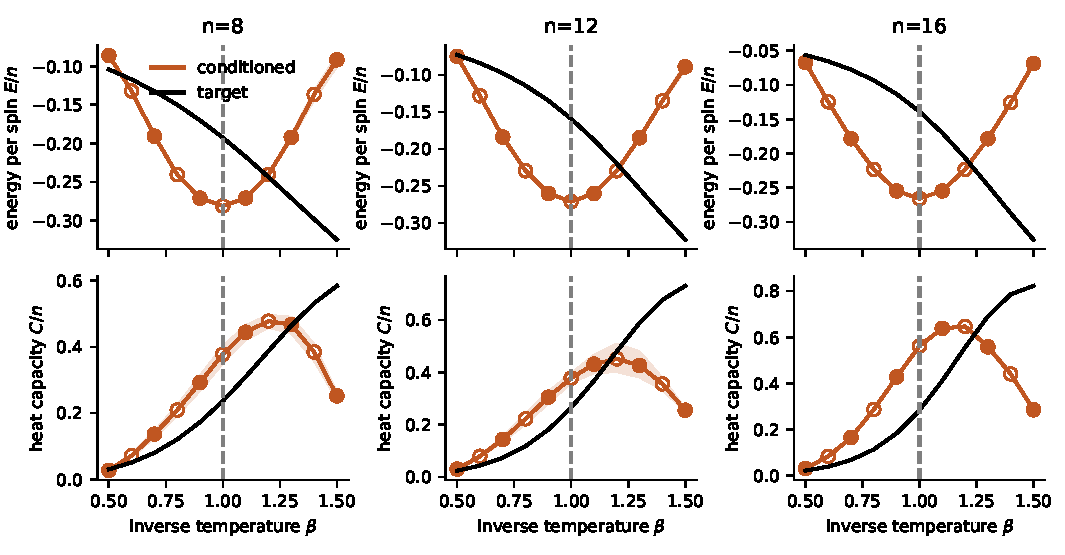
\includegraphics[width=\textwidth]{curie_weiss_figures/curie_weiss_thermodynamics.pdf}
\caption{Energy and heat-capacity response of the symmetry-aligned conditioned
circuit. Filled and hollow markers denote training and held-out temperatures;
bands are 95\% paired-bootstrap intervals over ten seeds. The vertical line
marks the unseen $\beta=1$ point.}
\label{fig:cw-thermodynamics}
\end{figure*}
\else
Curie--Weiss result tables are withheld until all 270 result envelopes,
checkpoints, and probability archives have matching digests.
\fi

\begin{table}[t]
\centering
\caption{Frozen data allocation in the condition-count study.}
\label{tab:data-allocation}
\begin{tabular}{rrrrr}
\toprule
$K$ & \multicolumn{2}{c}{fixed per condition} &
\multicolumn{2}{c}{fixed total}\\
 & train & validation & train & validation\\
\midrule
2 & 10,000 & 2,000 & 9,000 & 1,800\\
3 & 10,000 & 2,000 & 6,000 & 1,200\\
5 & 10,000 & 2,000 & 3,600 & 720\\
9 & 10,000 & 2,000 & 2,000 & 400\\
\bottomrule
\end{tabular}
\end{table}

\section{Complete factorial results}
\label{app:factorial}

Table~\ref{tab:factorial-all} reports every size--width cell.  Effects average
conditions within seed and then pair by seed.  Positive values favor the
conditioned model.  Status letters are S (95\% interval strictly positive), M
(contains zero), and U (strictly negative), ordered as training control,
held-out adjacent-reference oracle, and held-out coordinate-weighted mixture.  They describe the
observed uncertainty and do not implement a success rule.

\begin{table*}[t]
\centering
\scriptsize
\caption{All factorial profile-TVD effects with deterministic paired 95\%
bootstrap intervals.}
\label{tab:factorial-all}
\begin{tabular}{@{}rrp{0.20\textwidth}p{0.20\textwidth}
  p{0.20\textwidth}l@{}}
\toprule
$n$ & $s/\sqrt n$ & no condition $-$ conditioned &
adjacent-reference oracle $-$ conditioned &
mixture $-$ conditioned & S/M/U\\
\midrule
\tableinput{generated/factorial_cells.tex}
\bottomrule
\end{tabular}
\end{table*}

\ifgaussianresults
\begin{table*}[t]
\centering
\caption{Conditioned-model profile-TVD wins at the seed--Condition level in
every factorial cell.  Denominators are 50 Training comparisons and 80
Held-out comparisons per cell.}
\label{tab:factorial-wins}
\begin{tabular}{rrrrr}
\toprule
$n$ & $s/\sqrt n$ & vs. no condition & vs. adjacent-reference oracle & vs. mixture\\
\midrule
\tableinput{generated/factorial_wins.tex}
\bottomrule
\end{tabular}
\end{table*}
\fi

For auditability, the machine-readable report also records cell-level wins at
each seed--condition pair, mean and width error, exact Conditional MMD,
checkpoint selection, and model and target shell probabilities.  The complete
probability artifact retains all $2^n$ model probabilities at every declared
evaluation coordinate.

\section{Raw-bitstring diagnostics}
\label{app:bitstring}

Table~\ref{tab:bitstring-all} keeps the raw-law limitation adjacent to the
primary profile result.  Because targets are uniform within shells, profile
TVD is a quotient metric: it ignores redistribution within a shell.  The
difference between profile and bitstring TVD quantifies that unmodeled
structure.  A positive paired effect still means the conditioned model is
closer than the named baseline, but a large absolute TVD remains a limitation
even when the relative comparison is favorable.

\begin{table*}[t]
\centering
\scriptsize
\caption{Raw bitstring TVD across all factorial cells.  The middle columns are
the conditioned model's absolute mean TVD; effects are paired 95\% intervals.}
\label{tab:bitstring-all}
\begin{tabular}{@{}rrrrp{0.27\textwidth}p{0.27\textwidth}@{}}
\toprule
$n$ & $s/\sqrt n$ & training & held out & no condition $-$ conditioned &
adjacent-reference oracle $-$ conditioned\\
\midrule
\tableinput{generated/raw_bitstring_cells.tex}
\bottomrule
\end{tabular}
\end{table*}

\ifgaussianresults
\begin{table*}[t]
\centering
\scriptsize
\caption{Absolute secondary diagnostics for the conditioned model, averaged
over Conditions and seeds.  ``Train'' and ``held'' denote Training and
Held-out coordinates.}
\label{tab:secondary-all}
\begin{tabular}{@{}rrcccccc@{}}
\toprule
& & \multicolumn{2}{c}{mean absolute error} &
\multicolumn{2}{c}{width absolute error} &
\multicolumn{2}{c}{exact Conditional MMD}\\
$n$ & $s/\sqrt n$ & train & held & train & held & train & held\\
\midrule
\tableinput{generated/secondary_diagnostics.tex}
\bottomrule
\end{tabular}
\end{table*}
\fi

\section{Condition-count results}
\label{app:condition-count}

\ifgaussianresults
Table~\ref{tab:condition-count-all} reports both data regimes, the average and
worst held-out coordinate, parameter count, and optimization work.  The
shared-model parameter and update counts do not grow with $K$; the independent
reference collection's stored parameters and optimizer work grow linearly.
The per-condition JSON rows behind this table are retained so that a mean cannot hide a single
difficult coordinate.

\begin{table*}[t]
\centering
\scriptsize
\setlength{\tabcolsep}{3pt}
\caption{Condition-count and data-allocation results at $n=19,s=0.50$.}
\label{tab:condition-count-all}
\begin{tabular}{rlllrrrrr}
\toprule
$K$ & regime & train/condition & val./condition & mean & worst & params &
shared upd. & reference upd.\\
\midrule
\tableinput{generated/condition_count_cells.tex}
\bottomrule
\end{tabular}
\end{table*}

\begin{table*}[t]
\centering
\scriptsize
\setlength{\tabcolsep}{2.5pt}
\caption{Condition-count paired profile-TVD effects with 95\% intervals.
Positive control, adjacent-reference-oracle, and mixture effects favor conditioning; a
positive reference gap means the independent circuits have lower Training profile TVD.}
\label{tab:condition-count-intervals}
\begin{tabular}{@{}rlp{0.19\textwidth}p{0.19\textwidth}
  p{0.19\textwidth}p{0.19\textwidth}@{}}
\toprule
$K$ & Regime & no condition $-$ conditioned & conditioned $-$ reference &
adjacent-reference oracle $-$ conditioned & mixture $-$ conditioned\\
\midrule
\tableinput{generated/condition_count_intervals.tex}
\bottomrule
\end{tabular}
\end{table*}

Table~\ref{tab:condition-count-per-condition} exposes every held-out
coordinate rather than leaving those values only in the machine-readable
report.  Entries are ten-seed means of profile TVD; lower is better.

\tablecaption{Per-condition held-out profile TVD in the condition-count
study.}\label{tab:condition-count-per-condition}
\tablefirsthead{%
\toprule
$K$ & Regime & $c$ & Conditioned & No condition & Adjacent oracle & Mixture\\
\midrule}
\tablehead{%
\toprule
$K$ & Regime & $c$ & Conditioned & No condition & Adjacent oracle & Mixture\\
\midrule}
\tabletail{\midrule\multicolumn{7}{r}{Continued on next page.}\\}
\tablelasttail{\bottomrule}
\begin{supertabular}{@{}rp{0.18\textwidth}rrrrr@{}}
\tableinput{generated/condition_count_per_condition.tex}
\end{supertabular}
\else

\paragraph{Evidence status.}
The condition-count tables are generated only after all declared campaign
identities and exact evaluations are complete.

\fi

\section{Exhaustive paired intervals}

The following machine-generated table lists every diagnostic comparison, not
only the profile-TVD effects selected for the main text.  The replication unit
is always the matched optimizer seed; conditions are averaged before
resampling.

\tableinput{generated/all_intervals_paginated.tex}
\clearpage

\section{Archived Gaussian ablations}
\label{app:ablations}

The topology, encoding, and ancilla studies predate the frozen factorial and
are preserved as bounded ablations.  Their metrics are regenerated from the
archived JSON/NPZ pairs and are not pooled with the new campaign.  Complete
connectivity uses 190 phases at $n=19$; the lattice and heavy-hex banks use 48
and 39.  The symmetric-reupload comparison uses three matched seeds.  The
ancilla ladder uses $m\in\{0,1,2,3,5,7\}$ and compares each augmented model
with a visible-only matched-parameter control.

Permutation twirling replaces a raw sample $x$ by $\pi(x)$ for a uniformly
random qubit permutation $\pi$.  For an exchangeable target, this preserves
the Hamming-weight profile and makes the output uniform within each observed
shell in expectation.  It is therefore a legitimate target-symmetry-aware
post-processing baseline.  It is not a symmetry learned by the circuit, it
uses known target structure, and it is excluded from raw-circuit claims.

\section{Negative two-coordinate feasibility study}
\label{app:negative-width}

An archived eight-qubit pilot attempted to condition jointly on Gaussian
location and width.  Its frozen design required single-condition
representability before any shared-model or interpolation interpretation.  At
seed 0, the four single-condition bitstring TVDs were 0.3883, 0.3177, 0.2220,
and 0.0945.  The two narrow-width cells failed the declared capacity screen;
their width errors were 0.4659 and 0.1058.  The study stopped, so it supplies
no evidence for two-coordinate conditional generation.  We include it to mark
the boundary of the present one-coordinate claim and to prevent selective
reporting of only successful Gaussian variants.

\section{Campaign integrity and reproduction}
\label{app:reproduction}

The Gaussian campaign is isolated under
\texttt{results/gaussian-foundations-v1}.  The immutable manifest digest binds
the run plan; a source-tree digest binds the numerical core used by the
resource preflight and every result, while a companion dependency-closure
snapshot binds the encoder, ansatz, simulator, target, artifact, environment,
and lockfile sources.  Dataset archives record role,
derived seed, condition grid, master-pool hash, and split hash.  A result is
complete only when its envelope, checkpoint, and probability archive all
exist and their digests agree.  Reservations without a complete optimizer
state are never silently restarted.

From the repository root, the principal commands are:
\begin{verbatim}
uv sync --frozen
uv run python scripts/prepare_gaussian_campaign.py
uv run python scripts/run_gaussian_campaign.py preflight
uv run python scripts/freeze_gaussian_execution_source.py
uv run python scripts/run_gaussian_campaign.py run \
  --shard-count 5 --shard-index 0
uv run python scripts/summarize_gaussian_campaign.py
uv run python scripts/verify_gaussian_legacy.py
uv run python scripts/finalize_gaussian_claims.py
uv run python scripts/generate_gaussian_tables.py
uv run python scripts/plot_gaussian_campaign.py
uv run pytest -q
uv run ruff check src scripts tests
uv run python scripts/build_gaussian_arxiv_archive.py
uv run python scripts/audit_gaussian_release.py
uv run python scripts/prepare_curie_weiss_campaign.py
uv run python scripts/run_curie_weiss_campaign.py preflight
uv run python scripts/run_curie_weiss_campaign.py run \
  --shard-count 5 --shard-index 0
uv run python scripts/finalize_curie_weiss_campaign.py
uv run python scripts/plot_curie_weiss_campaign.py
\end{verbatim}
Shard indices 1--4 are executed analogously.  Re-running a completed shard
verifies and skips immutable outputs.  Report, claim, table, and figure
generators refuse partial campaign state.


\end{document}
